\documentclass[11pt,a4paper]{ivoa}
\input tthdefs

\title{IVOA DataLink}

% see ivoatexDoc for what group names to use here
\ivoagroup{DAL}

\author[http://www.ivoa.net/twiki/bin/view/IVOA/PatrickDowler]
       {Patrick Dowler}
\author[http://www.ivoa.net/twiki/bin/view/IVOA/FrancoisBonnarel]
       {Fran\c{c}ois Bonnarel}
\author[http://www.ivoa.net/twiki/bin/view/IVOA/LaurentMichel]
       {Laurent Michel}
\author[http://www.ivoa.net/twiki/bin/view/IVOA/MarkusDemleitner]
       {Markus Demleitner}
\editor[http://www.ivoa.net/twiki/bin/view/IVOA/PatrickDowler]
       {Patrick Dowler}

% \previousversion[????URL????]{????Concise Document Label????}
\previousversion{This is the first public release}

\newcommand{\blinks}{\{links\}}
\newcommand{\attval}[2]{#1={\allowbreak}{"}#2{"}}


\begin{document}


\begin{abstract}
This document describes the linking of data discovery metadata
to access to the data itself, further detailed metadata, related
resources, and to services that perform operations on the data. The web
service capability supports a drill-down into the details of a specific
dataset and provides a set of links to the dataset file(s) and related
resources. This specification also includes a VOTable-specific method
of providing descriptions of one or more services and their input(s),
usually using parameter values from elsewhere in the VOTable document.
Providers are able to describe services that are relevant to the records
(usually datasets with identifiers) by including service descriptors in
a result document.
\end{abstract}


\section*{Acknowledgments}

The authors would like to thank all the participants in DAL-WG discussions
for their ideas, critical reviews, and contributions to this document.


\section*{Conformance-related definitions}

The words ``MUST'', ``SHALL'', ``SHOULD'', ``MAY'', ``RECOMMENDED'', and
``OPTIONAL'' (in upper or lower case) used in this document are to be
interpreted as described in IETF standard RFC2119 \citep{std:RFC2119}.

The \emph{Virtual Observatory (VO)} is a
general term for a collection of federated resources that can be used
to conduct astronomical research, education, and outreach.
The \href{http://www.ivoa.net}{International
Virtual Observatory Alliance (IVOA)} is a global
collaboration of separately funded projects to develop standards and
infrastructure that enable VO applications.


\section{Introduction}

This specification defines mechanisms for connecting metadata about
discovered datasets to the data, related data products, and web services
that can act upon the data.

The {\em links\/} web service capability is a web service capability
for drilling
down from a discovered dataset identifier (typically an IVOA publisher
dataset identifier) to find details about the data files that can be
downloaded, alternate representations of the data that are available, and
services that can act upon the data (usually without having to download
the entire dataset). The expected usage is for DAL (Data Access Layer)
data discovery services (e.g.\ a TAP service \citep{2010ivoa.spec.0327D}
with the ObsCore \citep{2017ivoa.spec.0509L} data
model or one of the simple DAL services) to provide an identifier that
can be used to query the associated DataLink capability. The DataLink
capability will respond with a list of links that can be used to access
the data. Here we specify the calling interface for the capability and
the response, which lists the links and provides both concrete metadata
and a semantic vocabulary so clients can decide which links to use.

The {\em service descriptor resource\/}
uses the metadata features of VOTable to
embed service metadata along with tabular data, such as would be obtained
by querying a simple DAL data discovery service or a TAP service. This
service metadata tells the client how to invoke a service and, for those
registered in an IVOA registry, how to lookup additional information
about the service. The service provider can use this mechanism to tell
clients about services that can be invoked to access the discovered
dataset in some way: get additional metadata, download the data, or
invoke services that act upon the data files. These services may be
IVOA standard services or custom services from the data providers. The
current version provides no way to describe the output of a service,
but this may be added in a future (minor) revision of this specification.

We expect that the {\em service descriptor resource\/}
mechanism will be the primary way that clients will find and
use the {\em links\/} capability from data discovery
responses.


\subsection{The Role in the IVOA Architecture}

DataLink is a data access protocol in the IVOA architecture whose purpose
is to provide a mechanism to link resources found via one service to
resources provided by other services.

\begin{figure}[ht]
\centering
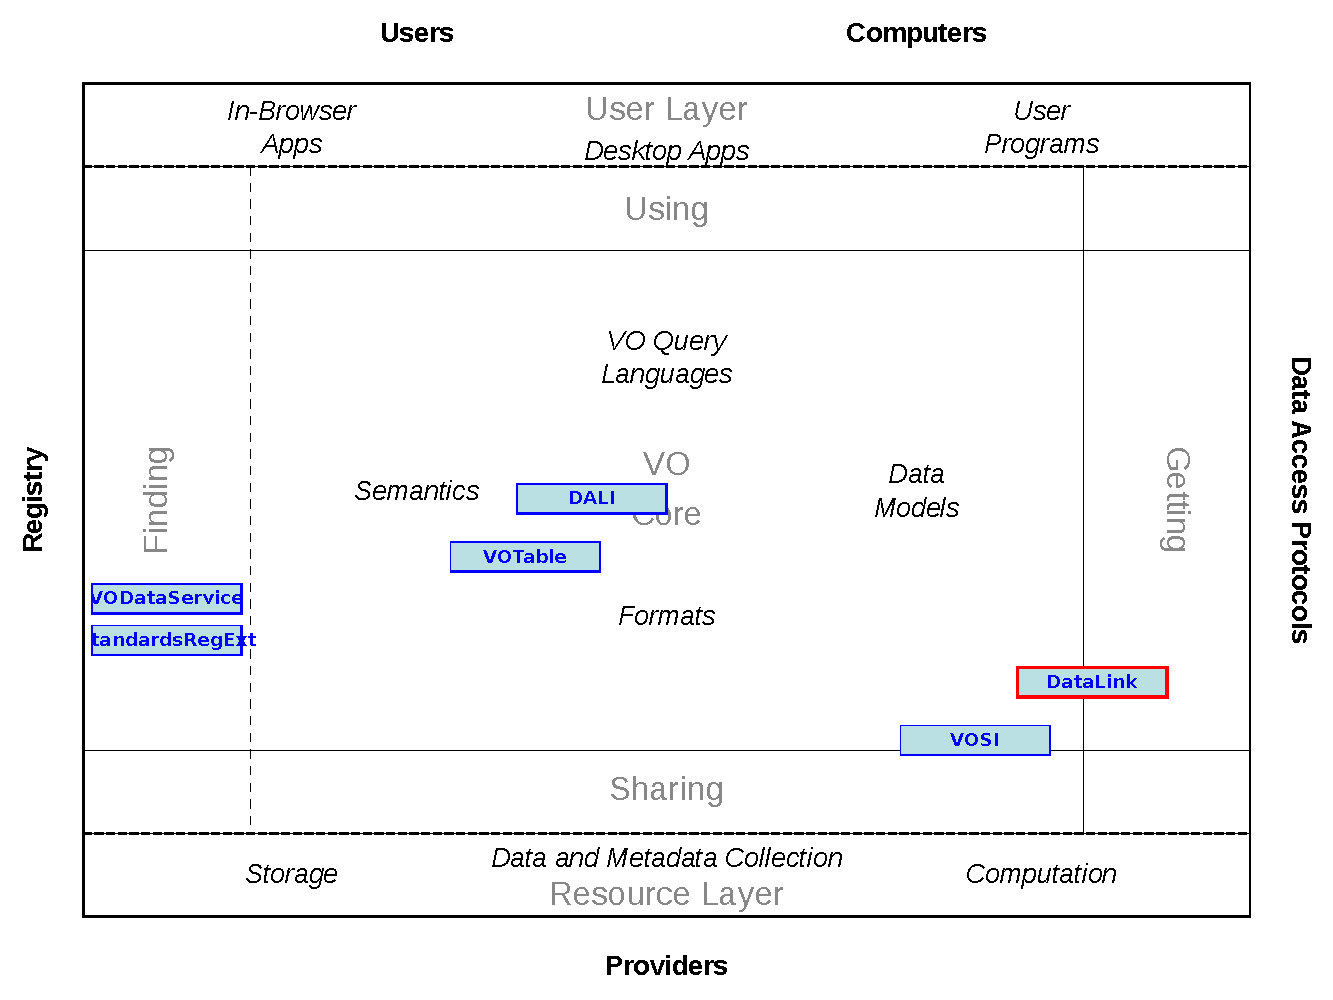
\includegraphics[width=0.9\textwidth]{role_diagram.pdf}
\caption{Architecture diagram for this document}
\label{fig:archdiag}
\end{figure}

Although not shown in Figure \ref{fig:archdiag},
any implementation of an access protocol could
make use of DataLink to expose resources. DataLink services conform to
the Data Access Layer Interface specification
(DALI, \citet{2013ivoa.spec.1129D}),
including the
Virtual Observatory Support Interfaces resources
(VOSI, \citet{2011ivoa.spec.0531G}).
DataLink services use VOTable \citep{2013ivoa.spec.0920O}
as the default output format both for successful
output and to return error documents.

DataLink specifies a standardID for itself, as defined in VODataService
\citep{2010ivoa.spec.1202P},
to be used in a StandardsRegExt record \citep{2012ivoa.spec.0508H}.
It also specifies how to
include standardID values in the response to describe links to services.

DataLink includes a description of how data discovery services can include
the link to the associated DataLink service in VOTable. VOTable is
also the default output format for the DataLink web service capability.


\subsection{Motivating Use Cases}

Below are some of the more common use cases that have motivated the
development of the DataLink specification. While this is not complete,
it helps to understand the problem area covered by this specification.


\subsubsection{Multiple Files per Dataset}
\label{sec:useMultiFile}

It is very common for a single dataset to be physically manifest as
multiple files of various types. With a DataLink web service, the client
can drill down using a discovered dataset identifier and obtain links to
download one or more data files.  For static data files, the DataLink
service will be able to provide a URL as well as the content-type and
content-length (file size) for each download.


\subsubsection{Progenitor Dataset}

In some cases, the data provider may wish to provide one or more links to
progenitor (input) datasets; this would enable the users to drill down
to input data in order to better understand the content of the product
dataset, possibly reproduce the product to evaluate the processing,
or reprocess it with different parameters or software.


\subsubsection{Alternate Representations}

For some datasets (large ones) it is useful to be able to access
preview data (either precomputed or generated on-the-fly) and use it
to determine if the entire dataset should be downloaded (e.g.\ in an
interactive session). A DataLink service can provide links to previews
as a URL with a specific relationship to the dataset and include other
metadata like content-type (e.g.\ image/png) and content-length to assist
the client in selecting a preview; multiple previews with different sizes
(content-length) could be returned in the list of links. Plots derived
from the dataset could also be linked as previews. Some previews may be
of the same content-type as the complete dataset, but reduced content
in some fashion (e.g.\ a representative image or spectrum derived from
a large data cube).

Links to alternate representations may be to pre-generated resources
or may be computed on the fly, using either an opaque URL or a custom
parameterised service (see \ref{sec:useCustom} below).

Other alternate representations that are not previews could also
be included in the list of links. For example, one could provide an
alternate download format for a data file with different content-type
(e.g.\ FITS and HDF).


\subsubsection{Standard Services}
\label{sec:useStandard}

Data providers often implement services that can access a dataset
or its files using standard service interfaces or provide alternate
representations of the dataset. For example, the links for a dataset
discovered via a TAP service could be to an SSA service, allowing
the caller to get an SSA query response that describes the same dataset
with metadata specific to the SSA service.

Providers should be able to link to current and future data
access services that perform filtering and transformations as these
services are defined and implemented (without requiring a new DataLink
specification). For IVOA standard services, the DataLink response would
use the VODataService standardID as the service type to tell the client which
standard (and version) the linked service complies to. The client can
select services they understand and use the link to invoke the service
(with additional service parameters added by the client).


\subsubsection{Free or Custom Services}
\label{sec:useCustom}

Data providers often implement custom services that can access a dataset
or its files or provide alternate representations of the dataset. The
availability of such services should be conveyed to clients/users in
the same fashion as for standard services. This allows services defined
within the VO to be used in conjunction with services defined outside
the VO to deliver features to users.


\subsubsection{Access Data Services}

In many access scenarios, server-side processing of data is
highly desirable, typically to reduce the amount of data to be
transferred. Examples for such operations are cutouts, slicing of
cubes, and re-binning to a coarser grid. Other examples for server-side
operations include on-the-fly format conversion or recalibration. For
the purpose of this specification, we call such services
{\em access data services}.
DataLink should let providers declare such access data services
in a way that a generic client can discover what operations are supported,
their semantics, and the domains of the operations' parameters. This lets
clients operate multiple independent access services behind a common user
interface, allowing scenarios like ``give me all voxels around positions
X in wavelength range Y of all spectral cubes from services Z\_1, Z\_2,
and Z\_9''.

Access data services may also be standard services or custom services;
at the time of writing, the definition of standard access service
capabilities is in progress in separate specifications.


\subsubsection{Recursive DataLink}

In some cases, a dataset may contain many files
(as in \ref{sec:useMultiFile} above)
and the provider may wish to make some files directly accessible and
other (less important) files only accessible via additional calls. Such
organisation of links could be accomplished by including a link to
another DataLink service in the initial DataLink response (e.g.\ recursive
DataLink). This service link would be described with both a service type
(as in \ref{sec:useStandard}) and content type.


\section{Resources}

The DataLink web service capability is implemented as an HTTP REST
\citep{std:RFC3986} web service capability
that conforms to the DALI-sync resource
description. The \blinks\ resource is described fully below
(see \ref{sec:linksResource}).
The values for the identifiers are typically found using a data
discovery service (e.g.\ TAP with ObsCore). Data discovery services that
work with an associated DataLink service should include a resource in
the discovery response to describe the DataLink service. The mechanism
for doing this is described below (see \ref{sec:serviceDescriptors}).

The requirements for a standalone DataLink service are given in the
table below.
\begin{center}
\begin{tabular}{|l|l|l|}
\sptablerule
{\bf resource type} & {\bf resource name} & {\bf required} \\
\sptablerule
\blinks             & service specific    & yes            \\
VOSI-availability   & /availability       & yes            \\
VOSI-capabilities   & /capabilities       & yes            \\
\sptablerule
\end{tabular}
\end{center}

A standalone DataLink service must have at least one \blinks\ resource;
it could have multiple \blinks\ resources (e.g.\ to support alternate
authentication schemes). Alternatively, the \blinks\ resource may be
embedded in another web service, in which case the VOSI-capabilities
resource of that service would also describe the \blinks\ capability.


\subsection{\blinks\ resource}
\label{sec:linksResource}

The \blinks\ resource is a synchronous web service resource that conforms
to the DALI-sync description. The implementer is free to name this
resource however they like as long as the \blinks\ resource is a sibling
of the VOSI resources; this restriction allows a client to construct
the URL to VOSI resources from any \blinks\ URL and thus discover other
capabilities or check the availablity if there is a failure. For example,
a DataLink service could have:
\begin{quote}
  \hspace*{-1.5em}
  {\small\nolinkurl{http://example.com/datalink/links}}
  --- anonymous access \\
  \hspace*{-1.5em}
  {\small\nolinkurl{http://example.com/datalink/auth-links}}
  --- HTTP authentication \\
  \hspace*{-1.5em}
  {\small\nolinkurl{https://example.com/datalink/links}}
  --- IVOA SSO authentication
\end{quote}

As a DALI-sync resource, the parameters for a request may be submitted
using an HTTP GET (query string) or POST action.


\subsubsection{ID}
\label{sec:resourceId}

The ID parameter is used by the client to specify one or more
identifiers. The service will return at least one link for each of the
specified values. The ID values are found in data discovery services
and may be readable URIs or opaque strings.

If an ID value specified by the client is not understandable by the
DataLink service, the service must include a single link in the output
with the ID and an error message (see below).

If the client submits more ID values than a service is prepared to
process, the service should process ID values up to the limit and
{\bf must} include an overflow indicator in the output
as described in DALI.
The service {\bf must not} truncate the output within the set of rows
(links) for a single ID value if the request exceeds such an input limit.

If the client submits no ID values, the service must respond with a
normal response (e.g.\ an empty results table for VOTable output).
The service may include service descriptors
(see \ref{sec:serviceDescriptors})
for related services and a service descriptor describing itself
(see \ref{sec:selfDescribing}).


\subsubsection{RESPONSEFORMAT}
\label{sec:responseformat}

The RESPONSEFORMAT parameter is described in DALI;
support for RESPONSEFORMAT is mandatory.

The only output format required by this specification is VOTable with
TABLEDATA serialization; services must support this format. Clients
that want to get the standard (VOTable) output format should simply
ignore this parameter.

To comply with this standard, a \blinks\ resource only needs to strip
off MIME type parameters and understand the following:
\begin{itemize}
  \item no RESPONSEFORMAT
  \item RESPONSEFORMAT=votable
  \item RESPONSEFORMAT=application/x-votable+xml
\end{itemize}
All of these result in the standard output format.

Service implementers may support additional output formats but must follow
the DALI specification if they chose any formats described there.


\subsection{Availability: VOSI-availability}

A DataLink web service must have a VOSI-availability resource,
as defined by DALI and VOSI.


\subsection{Capabilities: VOSI-capabilities}

A standalone DataLink web service must have a
VOSI-capabilities resource as defined by DALI and VOSI.
The standardID for the \blinks\ resource is
\begin{verbatim}
   ivo://ivoa.net/std/DataLink#links-1.0
\end{verbatim}

The following capabilities document shows the minimal metadata
and does not require a registry extension schema:
\begin{verbatim}
<?xml version="1.0" encoding="UTF-8"?>
<vosi:capabilities
   xmlns:vosi="http://www.ivoa.net/xml/VOSICapabilities/v1.0"
   xmlns:xsi="http://www.w3.org/2001/XMLSchema-instance"
   xmlns:vs="http://www.ivoa.net/xml/VODataService/v1.1">
  ...
  <capability standardID="ivo://ivoa.net/std/DataLink#links-1.0">
    <interface xsi:type="vs:ParamHTTP" role="std" version="1.0">
      <accessURL use="base">
        http://example.com/datalink/mylinks
      </accessURL>
      <queryType>GET</queryType>
      <queryType>POST</queryType>
      <resultType>
        application/x-votable+xml;content=datalink
      </resultType>
      <param std="true" use="required">
        <name>ID</name>
        <description>publisher dataset identifier</description>
        <ucd>meta.id;meta.main</ucd>
        <dataType>string</dataType>
      </param>
    </interface>
  </capability>
</vosi:capabilities>
\end{verbatim}

Multiple capability elements for the \blinks\ resource may be included;
this is typically used if they differ in protocol (http vs.\ https)
and/or authentication requirements.

The \blinks\ capability may also be included as a resource in another
service, in which case the VOSI-Capabilities for that service would
describe all the capabilities of that service, including \blinks.


\section{\blinks\ Response}

All responses from the \blinks\ resource follow the rules for DALI-sync
resources, except that the \blinks\ response allows for error
messages for individual input identifier values.


\subsection{DataLink MIME Type}
\label{sec:mime}

In some data discovery responses (e.g.\ ObsCore, \citet{2017ivoa.spec.0509L}),
there are columns
with a URL (access\_url in ObsCore) and a content type (access\_format in
ObsCore). If the implementation uses a DataLink service to implement this
data access, it should include a complete (including the ID parameter)
DataLink URL and a parameterised VOTable MIME type:
\begin{verbatim}
   application/x-votable+xml;content=datalink
\end{verbatim}
to denote that the response from that URL is a DataLink response.
This is also the MIME type for the \blinks\ response
(see \ref{sec:successfulRequests})
unless the caller has explicitly requested a specific value
via the RESPONSEFORMAT parameter (see \ref{sec:responseformat}).
Services may include other MIME type parameters in the response.


\subsection{List of Links}
\label{sec:listOfLinks}

The list of links that is returned by the \blinks\ resource can be
represented as a table with the following columns:
\begin{table}[h]
\begin{center}
\begin{tabular}{|l|p{0.29\textwidth}|l|l|}
\hline
{\bf name}      & {\bf description} & {\bf required} & {\bf UCD} \\
\hline
ID              & Input identifier & yes & meta.id;meta.main \\
\hline
access\_url     & link to data or service
                &          & meta.ref.url \\
\cline{1-2} \cline{4-4}
service\_def    & reference to a service descriptor resource
                & one only & meta.ref \\
\cline{1-2} \cline{4-4}
error\_message  & error if an access\_url cannot be created
                &          & meta.code.error \\
\hline
description     & human-readable text describing this link
                & yes & meta.note \\
\hline
semantics       & Term from a controlled vocabulary describing the link
                & yes & meta.code \\
\hline
content\_type   & mime-type of the content the link returns
                & no & meta.code.mime \\
\hline
content\_length & size of the download the link returns
                & no & phys.size;meta.file \\
\hline
\end{tabular}
\end{center}
\caption{Required Fields for Links}
\label{fig:linkFields}
\end{table}

All fields must be present in the output table; values must be provided
(or null) as described in Table \ref{fig:linkFields}. Each row in the table
represents one link and must have exactly one of:
\begin{itemize}
  \item an access\_url
  \item a service\_def
  \item an error\_message
\end{itemize}

If an error occurs while processing an ID value, there should be at least
one row for that ID value and an error\_message. For example, if an input
ID value is not recognised or found, one row with an error\_message
to that effect is sufficient.
If some links can be created (e.g.\ download links)
but others cannot due to some temporary failure (e.g.\ service outage),
then one could have one or more rows with the same ID and different
error\_message(s).

Services may include additional columns; this can be used to include
values that can be referenced from service descriptor input parameters
(see \ref{sec:serviceResources}).


\subsubsection{ID}

The ID column contains the input identifier value.


\subsubsection{access\_url}

The access\_url column contains a URL to download a single resource.
The URL in this column must be usable as-is with no additional
parameters or client handling; it can be a link to a dynamic
resource (e.g.\ preview generation).


\subsubsection{service\_def}

The service\_def column contains a reference from the result row to
a separate resource. This resource describes a service as specified
in section 4.
For example, if the response document includes this resource
to describe a service:
\begin{verbatim}
   <RESOURCE type="meta" utype="adhoc:service" ID="srv1">
   ...
   </RESOURCE>
\end{verbatim}
then the service\_def column would contain {\em srv1\/} to indicate that
a resource with XML ID srv1 in the same document describes the service.
Note that service descriptors do not always require an XML ID value;
it is only the reference from service\_def that warrants adding
an ID to the descriptor.


\subsubsection{error\_message}

The error\_message column is used when no accessURL can be generated for
an input identifier. If an error\_message is included in the output, the
only other columns with values should be the ID column and the semantics
column; all others should be null.


\subsubsection{description}

The description column should contain a human-readable description of
the link; it is intended for display by interactive applications.


\subsubsection{semantics}

The semantics column contains a single term from an external RDF
vocabulary that describes the meaning of this linked resource relative
to the identified dataset. The semantics column is intended to be
machine-readable and assist automating data retrieval and processing.

The core DataLink vocabulary defines a special term for
the concept of {\em this\/};
this term is used to describe links used for retrieval of the
dataset file(s). Since null values are not permitted, the semantics
value in cases where only an error\_message is supplied should be the
most appropriate for the link the service was trying to generate.

The value is always interpreted as a URI; if it is a relative URI,
it is resolved \citep{std:RFC3986} against the base URI of the
core DataLink vocabulary:
\begin{verbatim}
   http://www.ivoa.net/rdf/datalink/core
\end{verbatim}

The value used in the semantics column is normally the URI of the
vocabulary, followed by a fragment (\#), followed by a predicate from
the specified vocabulary.  For example, if the \blinks\ table contains a
link to a preview of a dataset, the ID column will contain the dataset
identifier, the access\_url column will contain the URL to the preview,
and the semantics column could contain this predicate:
\begin{verbatim}
   http://www.ivoa.net/rdf/datalink/core#preview
\end{verbatim}
or this relative URI:
\begin{verbatim}
   #preview
\end{verbatim}
For predicates outside the core DataLink vocabulary,
the full URI is required.

The core DataLink vocabulary is published at:
\begin{quote}
  \url{http://www.ivoa.net/rdf/datalink/core}
\end{quote}
and the latest version is available as a human readable document and an
RDF XML document. Services are encouraged to use the core vocabulary
as much as possible, but may use a custom vocabulary as long as they
use a custom vocabulary namespace (base URI); the base URI should be
resolvable to a human-readable document describing the terms.


\subsubsection{content\_type}

The content\_type column tells the client the general file format
(mime-type) they will receive if they use the link
(access\_url or invoking a service).
For recursive DataLink links, the content\_type value should
be as specified in section \ref{sec:mime}.
This field may be null (blank) if the value is unknown.


\subsubsection{content\_length}

The content\_length column tells the client the size of the download
if they use the link, in bytes. For VOTable, the FIELD must be
\attval{datatype}{long} with \attval{unit}{byte}.
The value may be null (blank)
if unknown and will typically be null for links to services.


\subsection{Successful Requests}
\label{sec:successfulRequests}

Successfully executed requests should result in a response with HTTP
status code 200 (OK) and a response in the format requested by the client
or in the default format for the service. The content of the response
(for tabular formats) is described above,
with some additional details below.

Unless the incoming request included a RESPONSEFORMAT parameter requesting
a different format, the content-type header of the response MUST be
``application/x-votable+xml'' with the
``content'' parameter set to ``datalink'',
with the canonical form given in \ref{sec:mime}
strongly recommended. Contrary to
all other uses of the string given in \ref{sec:mime},
clients wishing to evaluate
the content type of the response must, however, perform a full parse
of header value. This specification cannot and does not outlaw content
types with additional parameters
(e.g.\ ``application/x-votable+xml; content=datalink;charset=iso-8859-1'')
or with extra spaces or quotes
(as allowed for MIME types, \citet{std:RFC2045}).

If the incoming request includes a DALI RESPONSEFORMAT parameter,
content-type follows the DALI rules.


\subsubsection{VOTable output}

The table of links {\bf must} be returned in a RESOURCE with
\attval{type}{results}. The table {\bf must} be in TABLEDATA serialization
unless another serialization is specifically requested
(see \ref{sec:responseformat})
and supported by the implementation.
The name attribute for FIELD elements in the VOTable
(and the units in one case) are specified above (see \ref{sec:listOfLinks}).


\subsubsection{Other Output Formats}

This specification does not describe any other output formats, but allows
(via the RESPONSEFORMAT in section \ref{sec:responseformat})
implementations to provide
output in other formats.


\subsection{Errors}

The error handling specified for DALI-sync resources applies
to service failure (where no links can be generated) and to the usage
error where no ID parameter is specified. Services should return the
document format requested by the client (see \ref{sec:responseformat}).
For the standard
output format (VOTable) the error document {\bf must} also be VOTable.

For errors that occur while generating individual links, each
identifier may result in a link with only an error\_message
as described above.
In either case (error document or per-link error\_message),
the error message must start with one of the strings in
Table \ref{tab:errors}, in order of specificity.
\begin{table}[ht]
\begin{center}
\begin{tabular}{|l|l|}
\sptablerule
{\bf Error} & {\bf Meaning} \\
\sptablerule
NotFoundFault  & Unknown ID value    \\
UsageFault     & Invalid input (e.g.\ invalid ID value) \\
TransientFault & Service is not currently able to function \\
FatalFault     & Service cannot perform requested action \\
DefaultFault   & Default failure (not covered above) \\
\sptablerule
\end{tabular}
\end{center}
\caption{Error Messages}
\label{tab:errors}
\end{table}

In all cases, the service may append additional useful information to the
error strings above.
If there is additional text, it must be separated
from the error string with a colon (:) character, for example:
\begin{verbatim}
   NotFoundFault: ivo://example.com/data?foo cannot be found

   UsageFault: foo:bar is invalid, expected an ivo URI 
\end{verbatim}


\section{Service Descriptors}
\label{sec:serviceDescriptors}

The DataLink service interface is designed to add functionality to data
discovery services by providing the connection between the discovered
datasets and the download of data files and access to services that act
on the data. When the \blinks\ capability returns links to services, the
response document also needs to describe the services so that clients can
figure out how to invoke them. This is done by including an additional
metadata resource in the response document to describe each type of
service that can be used.

The same mechanism can also be used in any VOTable document, such
as a data discovery response from a TAP query or one of the simple
DAL query protocols, to enable clients to find and use the \blinks\
capability itself.

Here we describe how to construct a resource that describes a service
and add it to a VOTable document. The mechanism is general and can be
used wherever a VOTable document is created.


\subsection{Service Resources}
\label{sec:serviceResources}

In a data discovery response, one RESOURCE element (usually the first)
will have an attribute \attval{type}{results} and tabular data; this resource
contains the query result.

To describe an associated service, the VOTable would also
contain one or more resources with attribute \attval{type}{meta} and
\attval{utype}{adhoc:service}.
A resource of this type has no tabular data,
but may include a rich set of metadata. The utype attribute makes it
easy for clients to find the RESOURCE elements that describe services.
A service resource contains PARAM elements to describe the service and
a GROUP element with additional PARAM elements to describe the input
parameters.
The standard PARAM elements for a {\em service\/} resource
are described in Table \ref{tab:serviceParams}.
\begin{table}[h]
\begin{center}
\begin{tabular}{|l|l|l|}
\sptablerule
{\bf name}  &  {\bf value}  & {\bf required}  \\
\sptablerule
accessURL           & URL to invoke the capability   &  yes  \\
standardID          & URI for the capability         &  no   \\
resourceIdentifier  & IVOA registry identifier       &  no   \\
\sptablerule
\end{tabular}
\end{center}
\caption{Service Resource Parameters}
\label{tab:serviceParams}
\end{table}

For services that implement an IVOA standard, the standardID is specified
as the value attribute of the PARAM with \attval{name}{standardID}.
For free or custom services, this PARAM is not included.

For registered services, the resourceIdentifier PARAM allows the client
to query an IVOA registry for complete resource metadata. This could be
used to find documentation, contact info, etc. Although they need not be,
free or custom services could be registered in an IVOA registry and thus
have a resourceIdentifier to enable lookup of the record.

For standard services, the value of the accessURL PARAM must be the
accessURL for the capability specified by the standardID. The accessURL
is not generally usable as-is; the client must include extra parameters
as described below. If a standardID indicates a capability that supports
multiple HTTP verbs (GET, POST, etc.), the client may use any supported
verbs. Otherwise, there is no way in this version to specify that POST
(for example) is supported so clients should assume that only HTTP GET
may be used. Since the accessURL may contain parameters; clients must
parse the URL to decide how to append additional parameters when
invoking the service.

A GROUP with \attval{name}{inputParams} contains PARAM elements describing
how to invoke the service. For services where the parameter values
come from columns in the results resource, we use the ref attribute of
the PARAM to indicate the FIELD (column) with the values. Other PARAM
elements (without a ref attribute) are also allowed; these would describe
additional service parameters, the type of value that must be specified,
the meaning (UCD) of the value they apply to, etc.


\subsection{Example: Service Descriptor for the \blinks\ Capability}

The \blinks\ capability can be used with a result table when one of the
columns contains identifier values that can be used with the ID parameter
(see \ref{sec:resourceId}).
In order for the service resource to refer to this FIELD,
the FIELD element describing this column of the table
{\bf must} include an XML ID attribute
that uniquely identifies the FIELD (column).
For example, a response following the ObsCore-1.0 data model
would use the following:
\begin{verbatim}
   <FIELD name="obs_publisher_did" ID="primaryID"
          utype="obscore:Curation.PublisherDID"
          ucd="meta.ref.url;meta.curation"
          xtype="adql:VARCHAR" datatype="char" arraysize="256*" />
\end{verbatim}
where the ID value {\em primaryID\/} is arbitrary.
This FIELD would typically
be found within the RESOURCE of \attval{type}{results}. The same VOTable
document would have a second RESOURCE with \attval{type}{meta} to describe
the associated DataLink \blinks\ capability.

The \blinks\ capability described in section \ref{sec:linksResource}
is described by the following resource:
\begin{verbatim}
   <RESOURCE type="meta" utype="adhoc:service">
     <PARAM name="standardID" datatype="char" arraysize="*"
            value="ivo://ivoa.net/std/DataLink#links-1.0" />
     <PARAM name="accessURL" datatype="char" arraysize="*"
            value="http://example.com/mylinks" />
     <GROUP name="inputParams">
       <PARAM name="ID" datatype="char" arraysize="*"
              value="" ref="primaryID"/>
     </GROUP>
   </RESOURCE>
\end{verbatim}

Clients that want to find services to operate on the results would look
for resources with \attval{type}{meta} and \attval{utype}{adhoc:service}.
They would find a DataLink service specifically via the PARAM with
\attval{name}{standardID}. To call the service, the GROUP contains a PARAM
with the service parameter name and a ref attribute whose value is the
XML ID attribute on a FIELD. In the example above, the \attval{ref}{primaryID}
refers to the FIELD with \attval{ID}{primaryID} in the same document (usually
the result table). The URL to call the service would be:
\begin{verbatim}
   http://example.com/datalink/mylinks?ID=<obs_publisher_did value>
\end{verbatim}

Although this version of DataLink only has one parameter (ID), using a
GROUP and providing the service parameter name allows this recipe to be
used with any service and (with the GROUP) with multi-parameter services.

In the above example, the \blinks\ capability is not registered in an
IVOA registry so there is no resourceIdentifier PARAM included in the
descriptor.


\subsection{Example: Service Descriptor for an SIA-1.0 Service}

Suppose you have an SIA-1.0 service and you want users to be able to
call it to get SIA-1.0 specific metadata. This VOTable RESOURCE describes
the basic query interface of SIA-1.0:
\begin{verbatim}
   <RESOURCE type="meta" utype="adhoc:service">
     <PARAM name="resourceIdentifier" datatype="char" arraysize="*"
            value="ivo://example.com/mySIA" />
     <PARAM name="standardID" datatype="char" arraysize="*"
            value="ivo://ivoa.net/std/SIA#1.0" />
     <PARAM name="accessURL" datatype="char" arraysize="*"
            value="http://example.com/sia/query" />
     <GROUP name="inputParams">
       <PARAM name="POS" datatype="char" arraysize="*"
              value=""/>
       <PARAM name="SIZE" datatype="char" arraysize="*"
              value="0.5"/>
       <PARAM name="VERB" datatype="int" value="0"/>
       <PARAM name="FORMAT" datatype="char" arraysize="*"
              value="ALL">
         <VALUES>
           <OPTION value="ALL" />
           <OPTION value="image/fits" />
           <OPTION value="METADATA" />
         </VALUES>
       </PARAM>
     </GROUP>
   </RESOURCE>
\end{verbatim}

If this SIA service supported querying specific data collections via
a custom parameter named COLLECTION. The following PARAM describes the
custom parameter, including the possible values:
\begin{verbatim}
   <PARAM name="COLLECTION" datatype="char" arraysize="*"
          value="ALL">
     <VALUES>
       <OPTION value="ALL" />
       <OPTION value="FOO" />
       <OPTION value="BAR" />
     </VALUES>
   </PARAM>
\end{verbatim}
This PARAM would be added to the GROUP \attval{name}{inputParams}
of the service description.


\subsection{Example: Service Descriptor for VOSpace-2.0}

VOSpace-2.0 is a RESTful web service with several capabilities. Each of
these capabilities can be described with a service descriptor; this would
save the client having to perform a registry lookup to find and use the
service. The descriptors cannot describe the path usage and XML document
based input to the service, but they can describe the optional parameters:
\begin{verbatim}
   <RESOURCE type="meta" utype="adhoc:service" ID="vnodes">
     <PARAM name="resourceIdentifier"
            value="ivo://example.com/vospace" />
     <PARAM name="standardID"
            value="ivo://ivoa.net/std/VOSpace/v2.0#nodes" />
     <PARAM name="accessURL"
            value="http://example.com/vospace/nodes" />
     <GROUP name="inputParams">
       <PARAM name="detail" datatype="char" arraysize="*"
              value="min"/>
       <PARAM name="limit" datatype="integer"
              value="1000"/>
       <PARAM name="uri" datatype="char" arraysize="*"
              value=""/>
     </GROUP>
   </RESOURCE>
   <RESOURCE type="meta" utype="adhoc:service" ID="vtrans">
     <PARAM name="resourceIdentifier"
            value="ivo://example.com/vospace" />
     <PARAM name="standardID"
            value="ivo://ivoa.net/std/VOSpace/v2.0#transfers" />
     <PARAM name="accessURL"
            value="http://example.com/vospace/transfers" />
   </RESOURCE>
\end{verbatim}
Since the capability being described is RESTful and inputs are
{\em [?missing text?]}, the
caller must recognise the standardID values and use a VOSpace-aware
client to call the service.


\subsection{Example: Custom Access Data Service}

Parameters for custom access data services can be described such that
clients can figure out how to call the service and even create a basic
form-based user interface. The following Rotatable resource describes
a custom spectral cutout service:
{\small
\begin{verbatim}
   <RESOURCE type="meta" utype="adhoc:service" ID="apoadimo">
     <PARAM arraysize="*" datatype="char" name="accessURL"
            ucd="meta.ref.url"
            value="http://dc.zah.uni-heidelberg.de/flashheros/q/sdl/dlget"/>
     <GROUP name="inputParams">
       <PARAM arraysize="*" datatype="char" name="ID" ref="xjc7ra"
              ucd="meta.id;meta.main" value="">
         <DESCRIPTION>The pubisher DID of the dataset of interest
         </DESCRIPTION>
       </PARAM>

       <PARAM arraysize="*" datatype="char" name="FLUXCALIB"
              ucd="phot.calib" utype="ssa:Char.FluxAxis.Calibration"
              value="">
         <DESCRIPTION>Recalibrate the spectrum. Right now, the only
         recalibration supported is max(flux)=1 ('RELATIVE').
         </DESCRIPTION>
         <VALUES>
           <OPTION name="RELATIVE" value="RELATIVE"/>
           <OPTION name="UNCALIBRATED" value="UNCALIBRATED"/>
         </VALUES>
       </PARAM>

       <PARAM ID="axi5fg" datatype="float" name="LAMBDA_MIN"
              ucd="par.min;em.wl" unit="m" value="">
         <DESCRIPTION>Spectral cutout interval, lower limit
         </DESCRIPTION>
         <VALUES>
           <MIN value="3.4211e-07"/>
           <MAX value="5.5927e-07"/>
         </VALUES>
       </PARAM>

       <PARAM ID="k4dfpe" datatype="float" name="LAMBDA_MAX"
              ucd="par.max;em.wl" unit="m" value="">
         <DESCRIPTION>Spectral cutout interval, upper limit
         </DESCRIPTION>
         <VALUES>
           <MIN value="3.4211e-07"/>
           <MAX value="5.5927e-07"/>
         </VALUES>
       </PARAM>

       <PARAM arraysize="*" datatype="char" name="FORMAT"
              ucd="meta.code.mime" utype="ssa:Access.Format"
              value="">
         <DESCRIPTION>MIME type of the output format</DESCRIPTION>
         <VALUES>
           <OPTION name="FITS binary table"
                   value="application/fits"/>
           <OPTION name="Original format" value="image/fits"/>
           <OPTION name="Comma separated values" value="text/csv"/>
           <OPTION name="VOTable, tabledata encoding"
                   value="application/x-votable+xml;serialization=tabledata"/>
           <OPTION name="VOTable, binary encoding"
                   value="application/x-votable+xml"/>
           <OPTION name="Tab separated values"
                   value="text/tab-separated-values"/>
         </VALUES>
       </PARAM>
     </GROUP>
   </RESOURCE>
\end{verbatim}
}

The custom service described above supports 5 input parameters: ID,
FLUXCALIB, LAMBDA\_MIN, LAMBDA\_MAX, and FORMAT.

The PARAM describing the ID parameter has a ref attribute; the value is
the XML ID of a FIELD element in a results table in the same document
(the value {\em xjc7ra\/} is arbitrary;
it is an opaque string that matches
an ID value elsewhere in the document). The specified column contains
values for the ID parameter. The client (user) will pick rows (presumably
spectra) from the results table and then can invoke the service via the
ID parameter and value from that row.

The FLUXCALIB parameter allows the client to specify one of two values:
UNCALIBRATED or RELATIVE (listed as OPTIONS along with a description of
the meaning). The UCD \citep{2005ivoa.spec.0819D} value
of phot.calib conveys the basic meaning
of this parameter (it is related to photometric or flux calibration).

The LAMBDA\_MIN and LAMBDA\_MAX parameters allow the user to specify a
spectral interval to extract from the spectrum. The PARAM(s) specify that
the values are wavelengths:
\attval{ucd}{par.min;em.wl} and
\attval{ucd}{par.max;em.wl}
say they are minimum (par.min) and maximum (par.max) wavelength (em.wl)
values. The VALUES child elements convey a range of valid wavelength
values from which a subset could be extracted.

The FORMAT parameter allows the client to select from a list of output
formats for the extracted spectrum. Here, the name of the PARAM is
suitable to display (e.g.\ in a user interface) while the value would be
used to call the service.


\subsection{Example: Self-Describing Service}
\label{sec:selfDescribing}

A service may include a service descriptor that describes itself with
its normal output. This usage is comparable to prototype work on S3
(see \citet{note:s3})
and when combined with calling a service with no input parameters
(e.g.\ as allowed in \ref{sec:resourceId})
will make it easy for clients to obtain a
description of both standard and custom features.

The output of a \blinks\ capability with no input ID would include the
self-describing service descriptor and an empty results table:
\begin{verbatim}
   <RESOURCE type="meta" utype="adhoc:service" name="this">
     <PARAM name="standardID" datatype="char" arraysize="*"
            value="ivo://ivoa.net/std/DataLink#links-1.0" />
     <PARAM name="accessURL" datatype="char" arraysize="*"
            value="http://example.com/mylinks" />
     <GROUP name="inputParams">
       <PARAM name="ID" datatype="char" arraysize="*"
              value="" ref="primaryID"/>
     </GROUP>
   </RESOURCE>
   <RESOURCE type="results">
     <TABLE>
       <FIELD name="ID" datatype="char" arraysize="*"
              ucd="meta.id;meta.main" />
       <FIELD name="access_url" datatype="char" arraysize="*"
              ucd="meta.ref.url" />
       <FIELD name="service_def" datatype="char" arraysize="*"
              ucd="meta.ref" />
       <FIELD name="error_message" datatype="char" arraysize="*"
              ucd="meta.code.error" />
       <FIELD name="semantics" datatype="char" arraysize="*"
              ucd="meta.code" />
       <FIELD name="description" datatype="char" arraysize="*"
              ucd="meta.note" />
       <FIELD name="content_type" datatype="char" arraysize="*"
              ucd="meta.code.mime" />
       <FIELD name="content_length" datatype="long" unit="byte"
              ucd="phys.size;meta.file" />
       <DATA> <TABLEDATA/> </DATA>
     </TABLE>
   </RESOURCE>
\end{verbatim}

In the above example we give the self-describing service descriptor a
name attribute with the value ``this'' to indicate the self-describing
nature. This convention would make finding the self-description
unambiguous in cases where (i) the output also contained other service
descriptors and (ii) the caller could not infer which descriptor was
the self-describing one from the standardID (because it is optional
and not present for custom services and because they might just have a
URL). Even trying to match the URL that was used with the accessURL in
the descriptors is likely to be unreliable (e.g.\ if providers use HTTP
redirects to make old URLs work when service deployment changes).


\section{Changes}

This is the initial version of this document.


\subsection{PR-DataLink-1.0-20150413}

\begin{itemize}
\item
Restricted the \blinks\ resource path so that it must be a sibling of
the VOSI resources in order to allow discovery of VOSI resources from
a \blinks\ URL.
\item
Changed ID parameter to allow caller to invoke service with no ID values
and get an empty result table; this is actually easier to implement
than a special error case. Added reference to previous work on S3 and
an example section where an empty links response has a self-describing
service descriptor and an empty result.
\item
Fixed URL to DALI document in the references section.
\item
Fixed namespace prefix in example capabilities document to use recommended
value.
\end{itemize}


\subsection{PR-DataLink-1.0-20140930}

\begin{itemize}
\item
Re-organised introduction to introduce the links capability and
distinguish it from the service descriptor more clearly. Explicitly
noted that service descriptors do not describe the output of a service.
\item
Fixed various small typos mentioned on the RFC page.
\item
Clarified the use of the DataLink vocabulary in the semantics column of
the links table.
\item
Changed the links table output constraints to allow only one of:
access\_url, service\_def, or error\_message. This removes the possible
inconsistency of access\_url in the table being different from accessURL
in a service descriptor referenced by use of service\_def and reduces
service use by clients to a single supported approach.
\item
Added specific \attval{datatype}{long} to the content\_length field in the
links table.
\item
Moved VOSpace-2.0 service descriptor to be a separate example and made
it explicit that all the necessary details to invoke such a RESTful
service is not supported in this version of the specification; clients
must recognise the standardID to use RESTful web services.
\end{itemize}


\subsection{PR-DataLink-20140530}

\begin{itemize}
\item
Changed document status to proposed recommendation.
\item
Removed REQUEST parameter
\item
Added custom service example.
\item
Removed standard authentication and authorization error messages since
these are difficult to implement consistently in different web service
platforms. Changed the error message strings to use the word Fault
(following GWS-WG usage, e.g.\ VOSpace-2.0) since Error has specific
meaning in some platforms.
\end{itemize}


\subsection{WD-DataLink-20140505}

\begin{itemize}
\item
Changed the standardID for the \blinks\ resource to include version as
will be described in the StandardsRegExt record.
\item
Changed service descriptor resource to use
\attval{type}{meta} \attval{utype}{adhoc:service}
so VOTable documents pass schema validation and this resource type can
still be easily found.
\item
Improved the VOSI-capabilities example so it describes all parameters
of the example DataLink service.
\item
Removed unnecessary HTTP header advice and clarified the strict DataLink
mimetype usage.
\item
Removed mention of DALI-examples since it is an optional feature for
all services.
\item
Changed name of the input parameters group element in a service descriptor
to inputParams.
\item
Fixed reference to DALI document.
\item
Added SIA-1.0 resource desciptor example.
\item
Tried to clarify the relationship of the two aspects of DataLink in
the introduction.
\item
Specifically allow access\_url in the list of links to be different from
accessURL in the service descriptor, with VOSpace example.
\end{itemize}


\subsection{WD-DataLink-20140212}

\begin{itemize}
\item
Clarified that one can implement a standalone DataLink service or include
\blinks\ resources in other services.
\item
Re-ordered sections 2--5 so all the sections describing the
\blinks\ capability are together.
\item
Changed from GROUP with PARAM and FIELDref siblings to PARAM with ref
attribute when defining a parameter-column-with-values in section
\ref{sec:serviceResources}.
\item
Clarified the introduction so it is clear we intend to support linking
of any services via RESOURCE(s) in any responses.
\item
Changed the output of \blinks\ resource to clearly differentiate between
links with usable accessURL and links where the accessURL is a service
that requires more parameters. Changed the naming style for fields in
the list of links to use lower case with underscore separator so that
direct potential implementations don't run into case issues.
\end{itemize}



% \appendix
% \section{Changes from Previous Versions}
%
%
% these would be subsections "Changes from v. WD-..."
% Use itemize environments.


% NOTE: IVOA recommendations must be cited from docrepo rather than ivoabib
% (REC entries there are for legacy documents only)
\bibliography{ivoatex/ivoabib,ivoatex/docrepo,localrefs}


\end{document}
